\subsection{Normal VS Abnormal VS Artifact Model}
One of the primary concerns in applying machine learning models to the medical field is the potential 
consequence of misclassifying abnormal conditions as normal. Specifically, in the case of heartbeats, 
misclassifying an abnormal heartbeat as normal can have severe clinical implications. Therefore, 
our focus shifts from achieving the highest overall accuracy to minimizing the false positive rate (FPR) 
for the normal class. This approach ensures that fewer abnormal heartbeats are incorrectly classified as 
normal, thereby enhancing patient safety and diagnostic reliability.

\subsubsection{Methodology}
To effectively address the classification challenge, we categorized the heartbeats into three classes: 
normal, abnormal, and artifact, with the latter encompassing extrasystoles, murmurs, and extrahls. 
We then selected models from the previous section, prioritizing those with a low risk score. 
The features utilized were the filtered ones, and no class balancing was necessary since the classes 
were inherently balanced.

Each model was trained on 80\% of the dataset and tested on the remaining 20\%. 
The evaluation metrics included the ROC curve, macro F1 score, and balanced accuracy.


\subsubsection{Results}
The initial results are illustrated through the ROC curves for all the models. 
To handle the three-class problem, we employed the one-vs-rest strategy, where each class is compared 
against the other classes. Figure \ref{fig:ROC_normVSrest_allmodels} presents the ROC curves for 
the normal class versus the other classes across all models.


\begin{figure}[H]
    \centering
    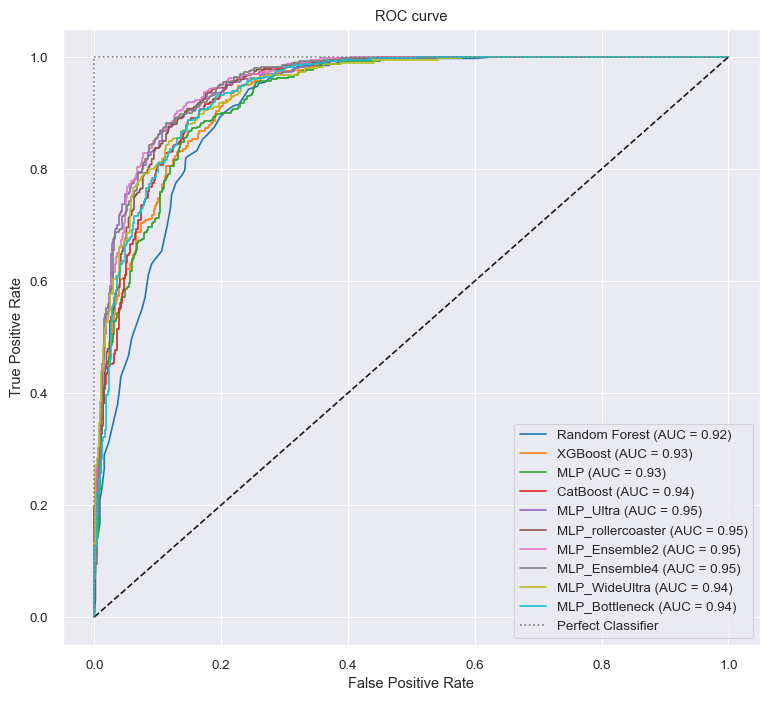
\includegraphics[width=1\columnwidth]{./images/ROC_normVSrest_allmodels.png}
    \caption{ROC curves of the normal class against the rest of the classes for all the models.}
    \label{fig:ROC_normVSrest_allmodels}
\end{figure}

\noindent
The results, as shown by the AUC values, indicate that the MLP model outperformed the others. Specifically, 
MLP\_Ultra, MLP\_Rollercoaster, MLP\_Ensemble2 and MLP\_Ensemble4 achieved the highest AUC values of 0.95.



